%\documentclass{article}
%\usepackage[utf8]{inputenc}

\documentclass[12pt]{article}
\usepackage{graphicx} % This lets you include figures
\usepackage{hyperref} % This lets you make links to web locations
\graphicspath{ {./images/} }

\usepackage[rightcaption]{sidecap}
\usepackage{subcaption}
\usepackage{wrapfig}
\usepackage{amssymb}
\usepackage{float}
\usepackage{amsmath}
\usepackage{imakeidx}

\makeindex


\title{Tropidance : Trajectory Optimization and Guidance}
\author{Sparsh Yadav}
\date{\today}

\begin{document}
\maketitle{}

\tableofcontents

\clearpage
\newpage

\section{Introduction}

Tropidance is an optimal control toolbox that enables the user to solve challenging trajectory optimization and guidance problems with ease, using direct optimal control techniques. With its ease of use, engineering teams can now get the results to complex optimal control problems rapidly. The potential for the software is limitless and can be used across multiple industries, including aerospace, robotics, energy, mobility and many more. 

Tropidance written in Python, one of the world's most popular programming language, currently implements several state-of-the-art computationally efficient MPSP algorithms developed at ASL Lab, Aerospace Engineering, Indian Institute of Science. The fact it is written in Python makes is platform agnostic, as long as the python interpreter is available, you can get started in less than no time. Tropidance is accompanied with detailed user and developer documentation. Built with extensibility in mind, the software follows a modular approach and can be extended to implement any number of algorithms.

\section{Class of Problems}

Numerous complex problems in engineering can be formulated as optimal control problems. Numberous optimal control problem can be formulated as:

\begin{equation}
J(\mathbf{x}(.), \mathbf{u}(.))=E\left(\mathbf{x}\left(t_{0}\right), \mathbf{x}\left(t_{f}\right)\right)+\int_{t_{0}}^{t_{f}} L(\mathbf{x}(t), \mathbf{u}(t)) d t
\end{equation}
Subject to 
\begin{equation}
\dot{\mathbf{x}}(t)=f(\mathbf{x}(t), \mathbf{u}(t))
\end{equation}
\begin{equation}
\mathbf{x}\left(t_{0}\right)= \mathbf{x_0} 
\end{equation}
\begin{equation}
\mathbf{x}\left(t_{f}\right)= \mathbf{x_f} 
\end{equation}
\begin{equation}
h(\mathbf{x}(t), \mathbf{u}(t)) \leq 0
\end{equation}

The techniques for solving such optimal control problems can be broadly classified into direct and indirect techniques.\\

Indirect methods rely on the first-order necessary conditions and Pontryagin's minimum principle. These methods lead to a two-point boundary value problem and try to find the optimal trajectories for the state and the control by solving the TPBVP. Indirect methods are computationally intensive and the control solution is an open-loop solution which is undesirable as it can not account for disturbances.

Alternatively, direct methods transform the optimal control problem into a non-linear constrained optimization problem by discretization of the control input and the system dynamics at finite grid points. Mode Predictive static programming falls into this category.


MPSP combines the philosophy of MPC and Adaptive Dynamic Programming to solve a class of finite-horizon optimal control problems. It is an iterative technique that starts from “guess history” of the control solution. This guess solution is iterated upon to achieve the objective of minimum control effort. The key advantage here is the computational efficiency i.e. the iterations can be calculated with very less computational load. 

The flow chart in Figure 1.\ref{fig:MPSPFlowchart} describes the iterative procedure of the algorithm.


\begin{figure}[h]
    \centering
    \includegraphics[width=0.9\textwidth]{img/MPSPFlowchart.png}
    \caption{Flowchart of the MPSP Algorithm}
    \label{fig:MPSPFlowchart}
\end{figure}


\section{MPSP Mathematical Background}

In regular MPSP, a general nonlinear system is considered ( in the discrete domain ), the state and output equations are given by

\begin{equation}
X_{k+1}=F_{k}\left(X_{k}, U_{k}\right) \\
Y_{k}=h_{k}\left(X_{k}\right)
\end{equation}

where $X \in \Re^{n}, U \in \Re^{m}, Y \in \Re^{p}$ and $k=1,2, \ldots, N$ are the time steps. The primary objective is to obtain a suitable control history $U_{k}, k=1,2, \ldots, N-1,$ so the output at the final time step $Y_{N}$ reaches a desired value $Y_{N}^{*}$ i.e. $Y_{N}^{*},$ i.e. $Y_{N} \rightarrow Y_{N}^{*}$

For mathematical development, the error is defined as $  \triangle Y_{N} \triangleq Y_{N}-Y_{N}^{*} $ Next, using small error approximation we get

\begin{equation}
\Delta Y_{N} \cong d Y_{N}=\left[\frac{\partial Y_{N}}{\partial X_{N}}\right] d X_{N}
\end{equation}

However, we can write the error in state at time $ (k+1)$ as

\begin{equation}
d X_{k+1}=\left[\frac{\partial F_{k}}{\partial X_{k}}\right] d X_{k}+\left[\frac{\partial F_{k}}{\partial U_{k}}\right] d U_{k}
\end{equation}
where $d X_{k}$ and $d U_{k}$ are the errors in state and control, respectively, at time $k$.

Expanding iteratively until $k=1$, we get

\begin{equation}
d Y_{N}=A d X_{1}+B_{1} d U_{1}+B_{2} d U_{2}+\cdots+B_{N-1} d U_{N-1}
\label{eq:dYEquation}
\end{equation}

where,
\begin{equation}\begin{aligned}
A & \triangleq\left[\frac{\partial Y_{N}}{\partial X_{N}}\right]\left[\frac{\partial F_{N-1}}{\partial X_{N-1}}\right] \cdots\left[\frac{\partial F_{1}}{\partial X_{1}}\right] \\
B_{k} & \triangleq\left[\frac{\partial Y_{N}}{\partial X_{N}}\right]\left[\frac{\partial F_{N-1}}{\partial X_{N-1}}\right] \cdots\left[\frac{\partial F_{k+1}}{\partial X_{k+1}}\right]\left[\frac{\partial F_{k}}{\partial U_{k}}\right], \quad k=1, \ldots, N-2 \\
B_{N-1} & \triangleq \left[\frac{\partial Y_{N}}{\partial X_{N}}\right]\left[\frac{\partial F_{N-1}}{\partial U_{N-1}}\right]
\end{aligned}\end{equation}

Equation \ref{eq:dYEquation} is solved with the cost function in \ref{eq:CostFunction} using static optimization techniques to get the update Equation \ref{eq:UpdateEquation} for the control, such that deviation at final-time is minimized.

\begin{equation}J=\frac{1}{2} \sum_{k=1}^{N-1}\left(U_{k}^{0}-d U_{k}\right)^{T} R_{k}\left(U_{k}^{0}-d U_{k}\right)
\label{eq:CostFunction}
\end{equation}

\begin{equation}U_{k}=U_{k}^{0}-d U_{k}=R_{k}^{-1} B_{k}^{T} A_{\lambda}^{-1}\left(d Y_{N}-b_{\lambda}\right), \quad k=1,2, \ldots,(N-1)
\label{eq:UpdateEquation}
\end{equation}

where,

\begin{equation}A_{\lambda} \triangleq\left[-\sum_{k=1}^{N-1} B_{k} R_{k}^{-1} B_{k}^{T}\right], b_{\lambda} \triangleq\left[\sum_{k=1}^{N-1} B_{k} U_{k}^{0}\right]
\end{equation}

\subsection{Why MPSP is computationally efficient?}
\begin{enumerate}
	\item A dynamic programming problem is converted to a static programming problem, and thus it requires only a static costate vector for the control update
	\item The symbolic costate vector has a closed-form solution, which reduces the computational load.
	\item The sensitivity matrices that are necessary to compute the static costate vector can be calculated recursively.
\end{enumerate}

\section{Applications of MPSP}
The algorithm's feasibility and efficiency has been demonstrated on several benchmarks (double integrator, Zermelo) and complex engineering problems. The focus here is on real-time aerospace applications.

\begin{itemize}
\item Aerospace Applications
	\begin{itemize}
		 \item Ascent phase guidance of ballistic missiles \cite{padhi2009model}
		 \item Guidance of interceptors with hard constraints \cite{dwivedi2011suboptimal,mondal2018angle}
		\item Guidance of solid-motor propelled flight vehicles \cite{kothari2010nonlinear}
		\item Guidance of solid-motor propelled flight vehicles with flexible final time  \cite{maity2016robust}
		\item Re-entry guidance of Reusable Launch Vechicles \cite{chawla2010suboptimal,halbe2014robust}
		\item Guidance of Air-launched missile to a predetermined target \cite{oza2012impact}
		\item Soft Lunar landing \cite{Sachan2019}
	\end{itemize}
\item Robotics
	\begin{itemize}
		\item Trajectory tracking for robotics \cite{kumar2019model}
		\item Inverted Pendulum \cite{mathavaraj2019unscented}
	\end{itemize}

\end{itemize}

In addition to the above applications, the algorithm is equally applicable to any area which necessitates the formulation of an optimal control problem, such as
\begin{itemize}
\item Biomedical: Artificial Pancreas
\item Electrical and Process Control
	
\end{itemize}

\iffalse
\section{Class of Porblems}
\subsection{Initial, final conditions known, and fixed final time}
MPSP as such tries to reduce the deviation at the final time $t_{f}$. 

\subsection{Flexible Final Time}
\subsection{Tracking Problem}
TMPSP

\fi

\section{A brief history of MPSP techniques}

\subsection{MPSP 2009}
MPSP combines the philosophy of non-linear model predictive control and approximate dynamic programming. The basic version of MPSP is applicable for finite-horizon non-linear problems with terminal constraints was presented in \cite{padhi2009model}. It brings the concept of trajectory optimization into guidance laws which are optimal in regards to the control effort required.

MPSP technique is computationally efficient and can be implemented online, providing for a wide range of real-time applications.  The effectiveness of the technique is demonstrated for the ascent phase guidance of a ballistic missile using solid motors in \cite{padhi2009model}.

\subsection{GMPSP 2014}
A generalized version of MPSP was presented in \cite{maity2014generalized} that extends upon the MPSP philosophy for solving a class of finite-horizon nonlinear optimal control problems with a hard terminal constraint. Two key features for its high computational efficiency include one-time backward integration of a small-dimensional weighting matrix dynamics, followed by a static optimization formulation that requires only a static Lagrange multiplier to update the control history. Moreover, it turns out that
under Euler integration and rectangular approximation of finite integrals it is equivalent to model predictive static programming technique \cite{padhi2009model}.

\subsection{QS-MPSP 2018}
Quasi-spectral MPSP was proposed in \cite{mondal2018angle} where the control variable is expressed as a weighted sum of basis functions. The coefficients of the basis functions are then determined using optimization techniques, in contrast, to control input at every grid point. This reduces the complexity of the problem and also ensures the smoothness of the control variable. Such a procedure also ensures the spread of the control over the available time to go.

QS-MPSP guidance was demonstrated in \cite{mondal2018angle} by formulating and solving an angle-constrained missile guidance problem to successfully engage an incoming high-speed ballistic missile target in three dimensions. The proposed QS-MPSP guidance showed considerable improvement in the lateral acceleration demand over the BPN guidance scheme.

\subsection{T-MPSP 2019}
A nonlinear optimal command tracking technique was presented in \cite{kumar2019model} called the Tracking-oriented MPSP. In this technique, like MPC a model-based prediction-correction approach is adopted.

In \cite{kumar2019model} TMPSP was used for trajectory tracking problem of a two-wheel differential drive mobile robot both in simulations and on real hardware. Successful results in both simulation and hardware implementation study demonstrated that the proposed, computationally efficient, T-MPSP algorithm can be implemented online and is promising for controlling dynamic systems under the paradigm of fast non-linear MPC.



  
\subsection{U-MPSP 2019}
Unscented MPSP was presented in \cite{mathavaraj2019unscented}, which applies to a class of problems where there are uncertainties in the time-invariant system parameters and/or initial conditions. This technique is a fusion of two recent ideas, namely MPSP and Riemann–Stieltjes optimal control problems. In UMPSP, first an unscented transform is utilized to construct a low-dimensional finite number of deterministic problems. The philosophy of MPSP is utilized next so that the solution can be obtained in a computationally efficient manner. The control solution not only ensures that the terminal constraint is met accurately with respect to the mean value, but it also ensures that the associated covariance matrix (i.e., the error ball) is minimized.

Significance of U-MPSP has been demonstrated in \cite{mathavaraj2019unscented} by successfully solving two benchmark problems, namely the Zermelo problem and inverted pendulum problem, which contain parametric and initial condition uncertainties.

\section{The MPSP Optimal Control Software Package }
The MPSP Optimal Control Software Package builds upon a decade of research into optimal control algorithms for real-time applications. The motivation of the package is to provide researchers, labs, and industry an easy to use, state-of-the-art Optimal Control problem solver. Anyone with a basic understanding of optimal control problem formulation will be able to use it. The package will include computationally efficient algorithms with mathematically proven convergence properties fit for real-time applications.

The source code of the package is developed generically with APIs provided to set up the problem and solve it. It is also ensured the code is developer-friendly, new functionality can be added to the code, as well as user friendly.

\subsection{Python Package}
Python has been chosen as the language to implementation of the optimal control package because of its widespread adoption and ease of use. Moreover, this language is extremely popular with academia and the industry as it a high-level language that provides for rapid testing and deployment. The language is also open-source and has a rich collection of scientific libraries.

The overall block diagram of the package is shown in Figure. \ref{fig:SoftwarePacakgeFlow}, which is subject to change as new modules are added.
\begin{figure}[h]
    \centering
    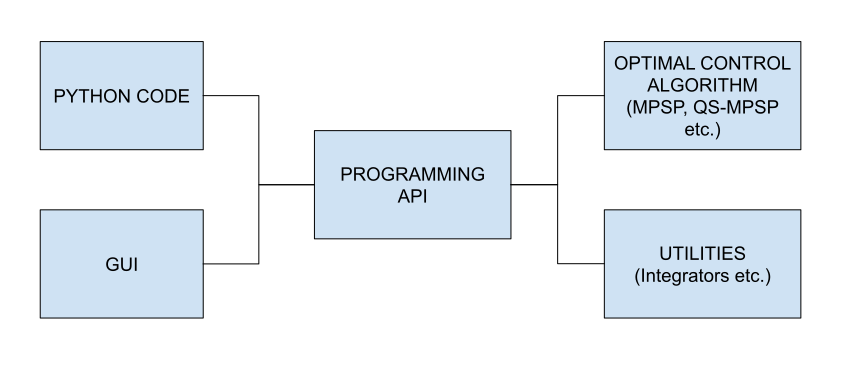
\includegraphics[width=0.9\textwidth]{img/CodeStructure.png}
    \caption{Block diagram of the software package.}
    \label{fig:SoftwarePacakgeFlow}
\end{figure}

\subsection{User Friendliness}

The aim of the software is collaboration and extensibility, these principles have been the guiding lights for the development. It should be easy for a newcomer to get started with the code and extend it to other algorithms.

The package provides an easy to use front-end API which can be used to define the model of the system, configure the algorithm and start the solution process. The solution process is straight forward as shown in Figure \ref{fig:CodeUsage}.

\begin{figure}[!htb]
    \centering
    \includegraphics[width=0.9\textwidth]{img/CodeUsage.png}
    \caption{Code sample to use the package.}
    \label{fig:CodeUsage}
\end{figure}

Salient points: 
\begin{itemize}
\item It is easy to configure the model and define the dynamics.
\item It is easy to configure a particular algorithm and its parameters. 
\item A simple front-end API for the user, that can be used for coding or to create a GUI. 
\item Providing verbose and descriptive messages to guide the user.
\item The code can be easily extended to include more functionality, using the principles of OOP (Object-oriented programming).
\item The aim is to write extensive tests for regression testing. 
\item Thorough documentation autogenerated with pydoc. 
\item Version Control using GIT.
\end{itemize}

\bibliographystyle{unsrt}
\bibliography{main}

%\href{http://class.guilford.edu/physics/dasmith}{this way}

%\footnote{You can put the link in a footnote like this.}

% Anything to the right of a percent sign will be ignored by LaTeX.
% You can use this to put notes to yourself.  If you want to actually
% get a percent sign in your PDF file, use \%.  This holds for many 
% symbols, like \$ and \&.  Without the backslash, LaTeX will think
% you are trying to give it a command, and it will get confused.
% Note that this paragraph does not show up in the PDF.

\listoffigures
\medskip
\end{document}
